\chapter{Theory}
\label{cha:theory}
\textit{by Olaf Kolditz and Uwe-Jens G�rke}

\begin{itemize}
	\item The idea of this chapter is to provide a brief-as-possible description (compendium-like) of governing equations for THM(C) processes in porous media. This is the theoretical basis for all benchmarks and examples upcoming part II and III of this book. There is a huge amount of literature available about Theory of Porous Medium (TPM). We will rather point to literature references than give any detailed derivations of the governing equations.
	\item will be refered to in the examples sections
	\item working equations (in the beginning of problem-type sections)
	\item list of symbols
\end{itemize}

From the mechanical point of view we consider non-isothermal flow of multiple fluid phases (compressible and incompressible fluids) in a deformable thermo-poro-elastic porous medium based on Biot's consolidation concept.
%
The followings steps are conducted
to derive the general field equations:
\begin{itemize}
 \item Macroscopic balance equations for mass, momentum and energy conservation of porous media (Section \ref{sec:balance_equations}),
 \item Constitutive relationships for non-isothermal multiphase processes in deformable porous media, 
 %(Section \ref{sec:constitutive_equations}),
 \item Applying the constitutive relationships and introducing physically based simplifications to the balance equations for the derivation of the general field equations. 
 %(Section \ref{sec:field_equations}).
\end{itemize}

%-------------------------------------------------------------------------
\section{Balance equations}
\label{sec:balance_equations}

%This section is a short reminder of the most important topics of textbook chapter 1 (\cite{Kol:2002}) condensed for the THM problem.

%.........................................................................
\subsection{Conservation principles}

The balance equations for mass, momentum and energy can be derived based on two fundamental principles.
%
In the
\textbf{Lagrangian formulation}\index{formulation - Lagrangian} we
follow the quantity along a pathline, i.e. following particles
(Fig. \ref{fig:Euler-Langrange}, top). In the \textbf{Eulerian
formulation}\index{formulation - Eulerian} of motion we consider
variations of the quantity with respect to a fixed control
volume\index{volume - control} at fixed places (Fig.
\ref{fig:Euler-Langrange}, bottom).

% *** EPS-Grafik ***
\begin{figure}[htb!]
\begin{center}
\footnotesize
%\includegraphics[height=5.973cm,width=11.507cm]{../figures/figure1.bmp}
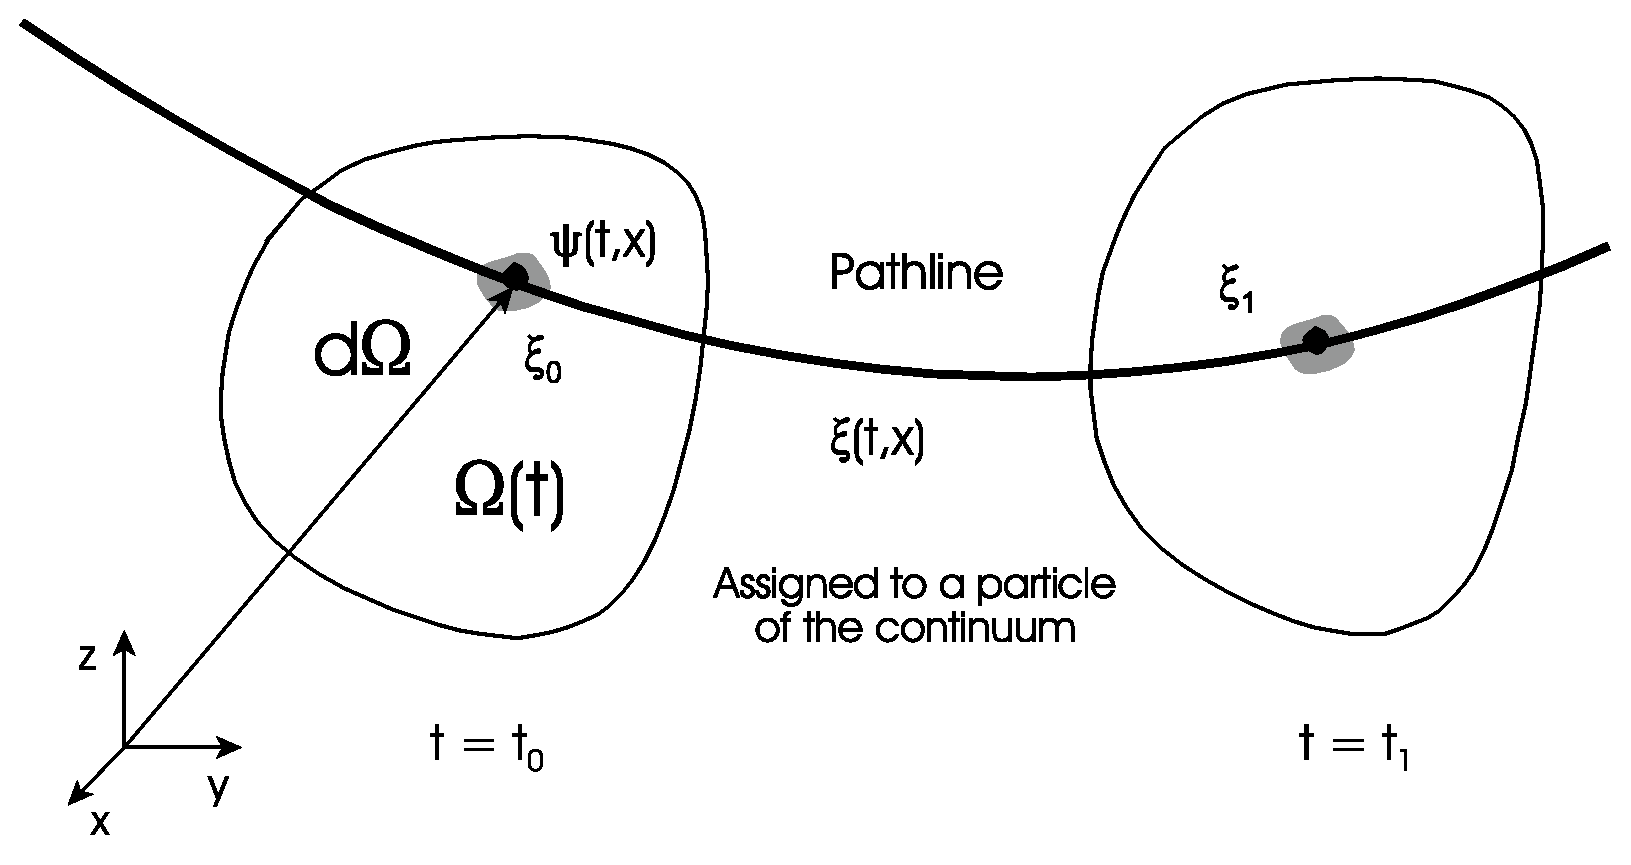
\includegraphics[width=0.8\columnwidth]{figures/mech1.eps}
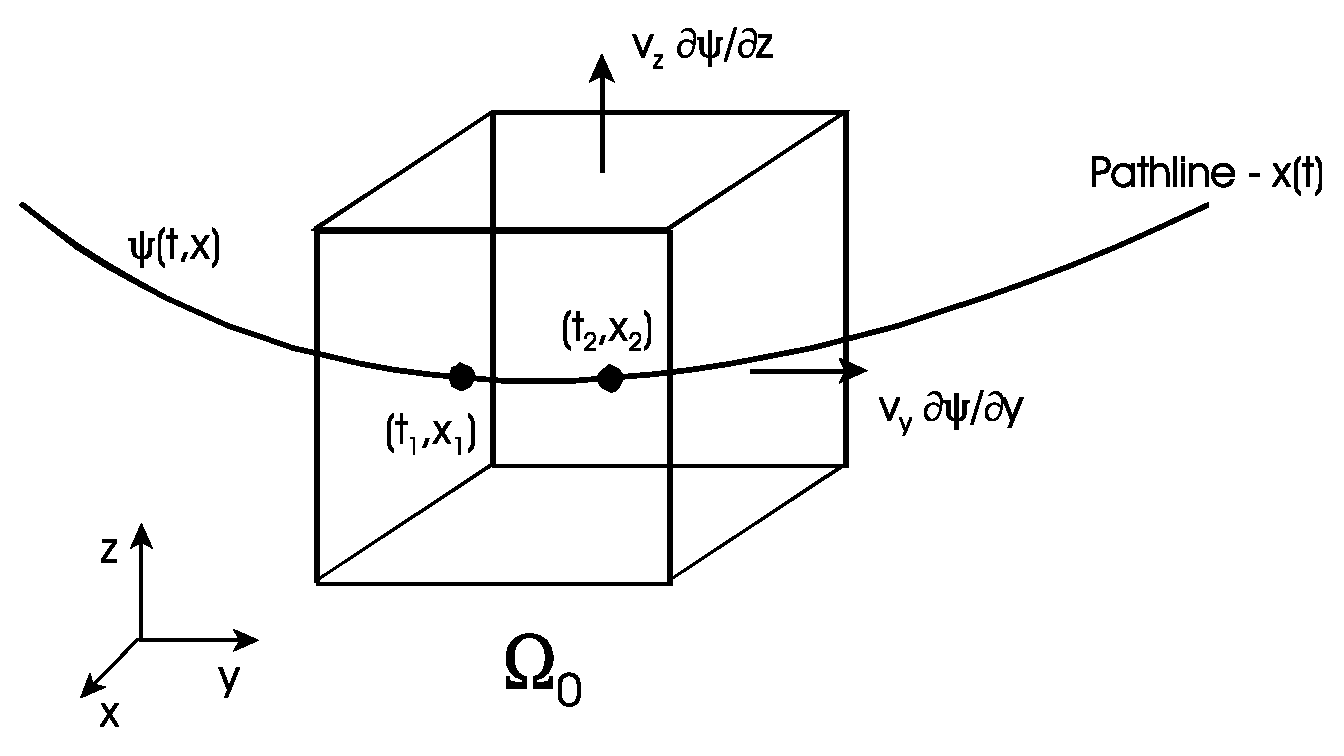
\includegraphics[width=0.8\columnwidth]{figures/mech2.eps}
\caption{Two basic descriptions of motion: Langrangian (top) and Eulerian (bottom) \cite{Kol:02}}
\label{fig:Euler-Langrange}
\end{center}
\end{figure}

Both conservation principles are related by two different forms of derivatives
\begin{equation}
\frac{d \psi}{dt}
=
\frac{\p \psi}{\p t} + \v\cdot\nabla\psi
\end{equation}
the total (or material) $d$ and partial derivitives $\p$, respectively.

The general balance equation is given by
%
\begin{eqnarray}
\frac{d}{dt} \int\limits_\Omega \psi d\Omega
=
\int\limits_\Omega
\left(
\frac{\partial\psi}{\partial t}
+
\nabla \cdot {\bf J}
\right)
d\Omega
=
\int\limits_\Omega Q^\psi d\Omega
\end{eqnarray}
%
where $\psi$ is the general conservation quantity (Tab. \ref{tab:conservation_quantities}), $\bf J$ is the general flux of $\psi$, and $Q$ is a source/sink term for $\psi$.
%
The corresponding extensive and intensive conservation quantities are summarized in Tab. \ref{tab:conservation_quantities}.

%
\begin{table}[htb!]
\caption{Conservation quantities}
\label{tab:conservation_quantities}
\begin{center}
\begin{tabular}{|ll|ll|}
\hline
Extensive  quantity &  Symbol    &  Intensive quantity      &  Symbol  \\
\hline \hline
%\mbox{\rule[1mm]{0cm}{3mm}Mass}
Mass                &  $M$,$M_k$ & Mass density             & $\rho$,$\rho_k$  \\
Linear momentum     &  $\bf m$   & Linear momentum density  & $\rho \bf v$ \\
Energy              &  $E$       & Energy density           & $e = \rho i + \frac 1 2 \rho v^2 $
\\[1pt]
\hline
\end{tabular}
\end{center}
\end{table}
%

\begin{itemize}
	\item Fluxes: diffusive, advective
\end{itemize}

\newpage
%.........................................................................
\subsection{Porous medium}

The Theory of Mixtures as one of the basic approaches to model the complex behavior of porous media has been developed (concerning basic assumptions see e.g. \cite{Bow:1976,TT:1960}). As the Theory of Mixtures does not incorporate any information about the microscopic structure of the material\footnote{Within the context of the Theory of Mixtures the ideal mixture of all constituents of a multiphase medium is postulated. Consequently, the realistic modeling of the mutual interactions of the constituents is difficult.}, it has been combined with the Concept of Volume Fractions by e.g. \cite{Bow:1980,BE:1986a,LS:1998,Pre:1980}. Within the context of this enhanced Theory of Mixtures (also known as Theory of Porous Media), all kinematical and physical quantities can be considered at the macroscale as local statistical averages of their values at the underlying microscale.
%
Concerning a detailed overview about the history of the modeling of the behavior of multiphase multicomponent porous media, the reader is referred to e.g. \cite{Boer:2000}. Comprehensive studies about the theoretical foundation and numerical algorithms for the simulation of coupled problems of multiphase continua are given in e.g. \cite{Boer:2000,EB:2002,LS:1998} and the quotations therein. 

\vspace{4cm}
\begin{figure}[htbp]
\hspace{3cm}
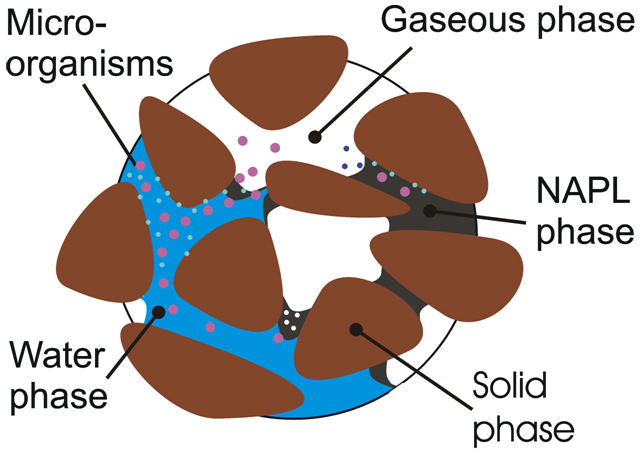
\includegraphics[width=0.06\columnwidth]{figures/pm.png}
\caption{Conceptual approach of a porous medium model}
\label{fig:pm1}
\end{figure}

The individual constituents $\varphi^{\alpha}$ of a porous material represent the phases of the overall aggregate or components within a phase. Below, $\alpha=s$ marks one immiscible solid phase (no sorption processes are considered), and $\alpha=\gamma$ denote several immiscible pore fluid phases. 
%
A porous medium, however, consists of multiple phases (fluids such as water, air and non-aqueous phase liquids (NAPLs) as well as solids). 
Moreover, these phases can contain several chemical components which can be dissolved in liquids or adsorbed to the solid phase (Fig. \ref{fig:pm1}).

Within the framework of the Concept of Volume Fractions, scalar variables like volume fractions and saturations are defined to describe the microstructure of a porous medium in a macroscopic manner neglecting the real topology and distribution of the pores. These variables serve as measures of local fractions of the individual constituents. The volume fractions $n^{\alpha}$ represent the ratio of the partial volume $dv^{\alpha}$ of a given constituent $\varphi^{\alpha}$ of a multiphase body with respect to the overall volume $dv$ of a representative elementary volume (REV) of the control domain $\Omega$ under consideration. Consequently, based on the definitions of the overall volume of the control domain
\begin{equation}
V=\int\limits_{\Omega}\,dv
\label{eq1}
\end{equation}
and the corresponding partial volumes of the individual constituents
\begin{equation}
V^{\alpha}=\int\limits_{\Omega}\,dv^{\alpha}\qquad\mbox{with}\qquad V=\sum\limits_{\alpha}\,V^{\alpha}
\label{eq2}
\end{equation}
the volume fractions
\begin{equation}
n^{\alpha}=\frac{dv^{\alpha}}{dv}
\label{eq3}
\end{equation}
provide some information about the local volume distribution of the individual constituents.
\begin{equation}
V^{\alpha}=\int\limits_{\Omega}\,dv^{\alpha}=\int\limits_{\Omega}\,n^{\alpha}\,dv
\label{eq4}
\end{equation}
One of the most characteristic media properties of a porous material is the porosity, the local amount of fluid volume fractions.
\begin{equation}
n=\sum\limits_{\gamma}\,n^{\gamma}=1\,-\,n^s
\label{eq5}
\end{equation}
Since, in general, the overall medium is completely filled with matter, from Eqn.~(\ref{eq2}) follows the saturation condition regarding the overall aggregate.
\begin{equation}
\sum\limits_{\alpha}\,n^{\alpha}=1
\label{eq6}
\end{equation}

If multiphase flow occurs, it is more convenient for various applications to use the (partial) fluid saturations $S^{\gamma}$ instead of the volume fractions. These local functions are given by
\begin{equation}
S^{\gamma}=\frac{dv^{\gamma}}{dv-dv^s}=\frac{n^{\gamma}}{n}
\label{eq7}
\end{equation}
obviously fulfilling the saturation condition regarding the pore content.
\begin{equation}
\sum\limits_{\gamma}\,S^{\gamma}=1
\label{eq8}
\end{equation}

Usually, constraint conditions addressing real physical effects are formulated to simplify complex mathematical and numerical models. Within the context of porous media, it is reasonable in most applications to assume the (material) incompressibility of constituents as a substantial constraint condition. The issue of (in)compressibility of a material is closely connected to the possible temporal evolution of its mass density.

Within the framework of the Concept of Volume Fractions, two different formulations of mass density related to the constituents of a porous medium are introduced. The so-called material (effective, realistic) density $\rho^{\alpha R}$ is defined as the ratio of the mass fraction $dm^{\alpha}$ of the given individual constituent $\varphi^{\alpha}$ with respect to its partial volume fraction.
\begin{equation}
\rho^{\alpha R}=\frac{dm^{\alpha}}{dv^{\alpha}}
\label{eq9}
\end{equation}
In contrast, the so-called partial (global, bulk) density is given by the ratio of the mass fraction of the constituent under consideration with respect to the volume fraction of the overall aggregate.
\begin{equation}
\rho^{\alpha}=\frac{dm^{\alpha}}{dv}
\label{eq10}
\end{equation}
Based on the definition of the volume fractions (\ref{eq3}), the material and the partial densities are correlated to each other.
\begin{equation}
\rho^{\alpha}=n^{\alpha}\,\rho^{\alpha R}
\label{eq11}
\end{equation}
If the volume fractions change with time under external loading, from Eqn.~(\ref{eq11}) follows that for an intrinsically incompressible individual constituent (constant material mass density) compressibility referred to the overall aggregate is observed.
\begin{equation}
\rho^{\alpha R}=\mbox{const} \quad\Rightarrow\quad
\rho^{\alpha}\,\neq\,\mbox{const}\quad\mbox{as}\quad n^{\alpha}\,\neq\,\mbox{const}
\label{eq12}
\end{equation}

Obviously, the mass density of the porous medium (homogenized overall aggregate) is defined as the sum of the partial densities of its constituents.
\begin{equation}
\rho=\sum\limits_{\alpha}\rho^{\alpha}
\label{eq13}
\end{equation}

The conceptual idea behind the formulations and relations presented above consists in the assumption that the mass fractions of all constituents of the multiphase medium are simultaneously present and statistically uniformly distributed over the entire control domain. Within this context, the material body under consideration is theoretically substituted by an aggregate completely and continuously filled by superimposed (overlapping) homogenized partial continua. In other words, all constituents of a porous medium are characterized as smeared substitute continua with reduced mass densities. Consequently, the motion and physics of the individual constituents as well as the overall aggregate can be specified by well-accepted phenomenological methods of continuum mechanics.

Describing the transport and deformation of the constituents of porous media within the framework of continuum mechanics it is assumed that the geometry of the control domain under consideration is characterized at each time by the solid skeleton, whereas the fluid pore content is able to flow across the boundary of the surface. This assumption serves as conceptual nucleus for the simulation of complex, coupled physical processes in multiphase porous media, particularly if a deformable solid skeleton is observed. Within this context, it proves to be reasonable not to model the absolute motion state of the pore content, but its motion relative to the motion of the solid phase, considering the porous medium as a local thermodynamic open system with the solid skeleton as volume under observation.

The macroscopic characterization of the physical processes considering the real microstructural situation in a statistically averaged manner is completely adequate for the most engineering, geotechnological and biomechanical problems under consideration (cf. \cite{GWASG:2006} and others).

%--------
\subsection{Phase mass balance}

We consider the mass balance of individual phases of a porous medium.
%
Neglecting mass exchange between the phases (no dissolution and sorption processes), the local mass balance for the individual constituent $\varphi^{\alpha}$ of the porous medium is given by
\begin{equation}
\frac{d_{\alpha}\rho^{\alpha}}{dt}+\rho^{\alpha}\,\nabla\cdot\mio{v}{\alpha}{}=
\frac{\partial\rho^{\alpha}}{dt}+\nabla\cdot\left(\rho^{\alpha}\mio{v}{\alpha}{}\right)=0
\label{eq14}
\end{equation}
with the velocity $\mio{v}{\alpha}{}$ of the constituent under consideration, and the usual divergence operator $\nabla\cdot()$. From the velocity-displacement relation for the solid skeleton follows
\begin{equation}
\mio{v}{s}{}=\mio{u}{s}{\dot}
\label{eq15}
\end{equation}
with the solid displacement vector $\mio{u}{s}{}$. The derivative
\begin{equation}
\frac{d_{\alpha}a}{dt}=\frac{\partial a}{dt}+\mio{v}{\alpha}{}\cdot\nabla a
\label{eq16}
\end{equation}
with the usual gradient operator $\nabla()$ denotes the material time derivative of an arbitrary variable $a$ with respect to the motion of a material point of the constituent $\varphi^{\alpha}$. It consists of a local (diffusive) part and a convective part associated with the velocity of the constituent.

As mentioned above, the transport processes of the fluid constituents of a porous medium are considered as their relative motion with respect to the motion of the deformable solid skeleton. Consequently, the relations between the material time derivatives (here, of an arbitrary variable $a$) with respect to the solid skeleton, and with respect to the individual fluid constituent $\varphi^{\gamma}$ is of crucial interest in terms of a unified numerical characterization of the different processes.
\begin{equation}
\frac{d_{\gamma}a}{dt}=\frac{d_{s}a}{dt}+\mio{v}{\gamma s}{}\cdot\nabla a
\label{eq17}
\end{equation}
Here, $\mio{v}{\gamma s}{}=\mio{v}{\gamma}{}-\mio{u}{s}{\dot}$ is the so-called seepage velocity describing the fluid motions with respect to the deforming skeleton material.

According to the generalized formulation~(\ref{eq14}), considering Eqns.~(\ref{eq5}) and (\ref{eq11}), the local solid phase mass balance is given by
\begin{equation}
\frac{d_s\left[(1-n)\rho^{sR}\right]}{dt}+(1-n)\,\rho^{sR}\,\nabla\cdot\mio{u}{s}{\dot}=0
\label{eq18}
\end{equation}
Following the same procedure, additionally considering Eqns.~(\ref{eq7}) and (\ref{eq17}), the mass balance relations for the fluid constituents $\varphi^{\gamma}$ with
\begin{equation}
\gamma\,=\,\mathrm{CO}_2,\,l
\label{eq19}
\end{equation}
can be defined with respect to the solid phase motion.
\begin{equation}
\frac{d_s\left(nS^{\gamma}\rho^{\gamma R}\right)}{dt}+
\nabla\cdot\left(nS^{\gamma}\rho^{\gamma R}\mio{v}{\gamma s}{}\right)+
nS^{\gamma}\rho^{\gamma R}\nabla\cdot\mio{u}{s}{\dot}=0
\label{eq20}
\end{equation}
Assuming material incompressibility of the solid phase, i.e. $d_s\rho^{sR}/dt\!\!=\!\!0$, and applying the solid phase mass balance~(\ref{eq18}), Eqn.~(\ref{eq20}) can be represented in a more detailed description.
\begin{eqnarray}
& & 
nS^{\gamma}\frac{d_s\rho^{\gamma R}}{dt}+n\rho^{\gamma R}\frac{d_sS^{\gamma}}{dt} \nonumber \\[1.5ex]
& & \quad
+\nabla\cdot(\rho^{\gamma}\mio{w}{\gamma s}{})+S^{\gamma}\rho^{\gamma R}\nabla\cdot\mio{u}{s}{\dot}=0
\label{eq21}
\end{eqnarray}
Here
\begin{equation}
\mio{w}{\gamma s}{}=nS^{\gamma}\mio{v}{\gamma s}{}
\label{eq22}
\end{equation}
is usually known as filter velocity of the motion of the pore fluid constituent $\varphi^{\gamma}$.

\begin{itemize}
	\item selection of primary variables
\begin{align}
d\rho (p,T)
=
\frac{\p \rho}{\p p} dp + \frac{\p \rho}{\p T} dT
\label{eqn:}
\end{align}
\end{itemize}

%.........
\subsubsection{Non-isothermal compositional two-phase flow in a deformable porous medium}

componental multi-phase formulation with respect to component $k$

\begin{align}
\frac{\p}{\p t}
\sum_\gamma \epsilon^\gamma \rho_k^\gamma
+
\nabla\cdot
\sum_\gamma \epsilon^\gamma \J_k^\gamma
+
\sum_\gamma \epsilon^\gamma \rho_k^\gamma \nabla\dot\u^s
=
\sum_\gamma \epsilon^\gamma Q_k^\gamma
\label{eqn:}
\end{align}

where $\epsilon^\gamma$ is the volume fraction of phase $\gamma$, e.g. $\epsilon^g = n S^g$.

\begin{itemize}
	\item selection of primary variables
\begin{align}
\frac{\p \epsilon^\gamma \rho_k^\gamma}{\p t}
=
\epsilon^\gamma
\left(
\frac{\p \rho_k^\gamma}{\p p} \frac{\p p}{\p t} 
+ 
\frac{\p \rho_k^\gamma}{\p T} \frac{\p T}{\p t} 
\right)
+
\rho_k^\gamma
\left(
\frac{\p \epsilon^\gamma}{\p p} \frac{\p p}{\p t} 
+ 
\frac{\p \epsilon^\gamma}{\p T} \frac{\p T}{\p t} 
\right)
\label{eqn:pv1}
\end{align}
\end{itemize}

%.........
\subsubsection{Non-isothermal consolidation}

Deformation processes in porous media are described by the momentum balance equation in terms of the total Cauchy's stress tensor $\miu{\sigma}{}{}$, which is additively decomposed into several partial stresses according to different physical events. The specific local overall linear momentum balance equation is given as follows:
%
\begin{eqnarray}
\nabla\cdot\left[
\phantom{\left(\fourtens{I}\right)}\!\!\!\!\!\!\!\!\!\!\!\!
\mio{\sigma}{\prime}{}\right. & - & \chi\left(S_{\mathrm w}\right)\,p_{\mathrm w}\,\miu{I}{}{}
\,-\,\miu{\sigma}{\mathrm{sw}}{}
\nonumber \\[1.5ex]
& - & \left.\alpha\,\Delta T\,\left(\fourtens{C}\ccdot\miu{I}{}{}\right)
\right]
\,+\,\rho\,\miu{g}{}{}\,=\,\miu{0}{}{}
\label{eq:4}
\end{eqnarray}
%
The representation Eq.~(\ref{eq:4}) of the stress decomposition is based on a modified effective stress law presented in \cite{RBCetal:2001}, where $\mio{\sigma}{\prime}{}$ is the macroscopic effective stress tensor, $\chi$ is the saturation dependent effective stress parameter of Bishop's type \cite{BB:1963}, $\miu{\sigma}{\mathrm{sw}}{}$ denotes the swelling stress, $\alpha$ is the thermal expansion coefficient, $\miu{I}{}{}$ represents the second-order identity tensor, $\fourtens{C}$ is the fourth-order elastic material tensor, which will be discussed later, and $\mio{g}{}{}$ is the gravity vector. 

%.........
\subsubsection{Heat transport}

\begin{eqnarray}
\sum_\gamma \epsilon^\gamma c^\gamma \rho^\gamma \frac{\p T}{\p t}
+
\nabla\cdot
(
\sum_\gamma \rho^\gamma \v^\gamma c^\gamma T - \sum_\gamma \epsilon^\gamma \lambda^\gamma \nabla T
)
= 
\sum_\gamma \epsilon^\gamma \rho^\gamma Q_h^\gamma + \v\cdot\nabla\sigma
\label{eqn:heat_transport}
\end{eqnarray}

%-------------------------------------------------------------------------
\section{Constitutive equations}
\subsection{Fluid properties}
\textit{by Norbert B�ttcher}

%-------------------------------------------------------------------------
\section{Coupled processes}

The below Tab. \ref{tab:coupled_phenomena} shows some of the important coupling phenomena during THMC processes in porous media. Among the modeling challenges in this field are following topics
\begin{description}
	\item[T:] Temperature depending material properties and reaction rates,
	\item[H:] Multi-phase flow with phase changes coupled to reactive transport,
	\item[M:] Cracking due to gas pressure, thermal stresses, de-saturation,
	\item[C:] Gas production, pore space clogging dur to precipitation.
\end{description}

\begin{table}[htb!]
\caption{Thermal coupled phenomena}
\label{tab:coupled_phenomena}
\begin{center}
\begin{tabular}{|l|l|l|l|}
\hline
\textbf{T} & TH & TM & TC \\
dependent  & Vapor flux        & Thermal stress  & Partial pressure (T) \\
parameters & Convection        & Cracking        & Reaction rates \\
\hline
HT & \textbf{H} & HM & HC \\
Advection & & Consolidation   & Advection \\
          & & Swelling stress & Partial pressure (p) \\
\hline
MT & MH & \textbf{M} & MC \\
   & Consolidation & & Pressure solution \\
   & Cracking      & & \\
\hline
CT & CH & CM & \textbf{C} \\
Reaction heat & Convection & Chemical damage & \\
\hline
\end{tabular}
\end{center}
\end{table}
%
